\documentclass{article}
\usepackage[catalan]{babel}
\usepackage[utf8]{inputenc}
\usepackage[T1]{fontenc}
\usepackage{graphicx}
\graphicspath{ {images/} }
\setlength{\parindent}{0cm}
\frenchspacing
\begin{document}
\title{PAC3: Control de Versions i Documentació} 
\author{Josep Turón i Viñas}
\date{Desembre del 2015}
\maketitle
\newpage
\section{Introducció}
Aquest document, realitzat amb \LaTeX, explica de forma detallada com s'ha portat a terme la resolució de la PAC 3: Control de Versions i Documentació, de l'assignatura optativa Desenvolupament de Programari, corresponent al Màster Universitari en Programari Lliure.\bigskip

En la primera part, s'explicarà com s'ha creat un dipòsit utilitzant Git amb els fitxers de filtres utilitzats en les pràctiques anteriors.\bigskip

En la segona part, s'explicarà com s'ha realitzat la documentació del codi dels filtres, utilitzant Doxygen, i finalment com s'ha redactat l'explicació de la PAC amb LaTeX. \bigskip

Finalment es presentaran unes breus Conclusions sobre el desenvolupament de la pràctica.\bigskip

Aquest document s'entregarà en format tex, dvi (propi del visor de textos xdvi) i pdf, juntament amb el fitxer de log de la compilació del fitxer tex. Tots aquests s'adjuntaran dins el fitxer PAC3.tar.gz juntament amb tots els altres fitxers generats durant el desenvolupament de la PAC.\bigskip

Un cop descomprimit el fitxer PAC3.tar.gz es generarà la següent estructura de directoris:
\begin{itemize}
\item /PAC3: conté el fitxer configdoxy de configuració de Doxygen.

\item /PAC3/libsrc: conté els fitxers amb el codi de les funcions filtres.c i la capçalera filtres.h.

\item /PAC3/doc: conté la documentació del codi dels filtres generada amb Doxygen i exportada en format HTML i LaTex.

\item /PAC3/descripcio\_proces: conté la documentació generada amb LaTex amb l'explicació del desenvolupament de la pràctica, en formats tex, dvi i pdf (aquest fitxer).

\item /PAC3/.git: conté el dipòsit de Git (directori ocult).
\end{itemize}
\newpage
\section{Control de Versions}
Per començar hem instal·lat les eines \textbf{git} i \textbf{gitk} (aquesta ens permet visualitzar el contingut del dipòsit i els \textit{commit} realitzats de forma gràfica), executant les comandes:\bigskip

\qquad sudo apt-get install git\bigskip

\qquad sudo apt-get install gitk\bigskip

A continuació configurem l'usuari, el seu correu electrònic, i un editor de textos per defecte. Així mateix podríem definir altres eines, que no necessitarem en aquesta pràctica:\bigskip

\qquad git config user.name Josep\bigskip

\qquad git config user.mail jturonv@uoc.edu\bigskip

\qquad git config core.editor vim\bigskip

Ara ja podem crear el dipòsit fent:\bigskip

\qquad git init\bigskip

I afegir els dos fitxers que volem a l'\textit{staging area}:\bigskip

\qquad git add libsrc/filtres.c\bigskip

\qquad git add libsrc/filtres.h\bigskip

o simplement pujant el directori:\bigskip

\qquad git add libsrc\bigskip

Amb la comanda\bigskip

\qquad git status\bigskip

veiem que tenim els dos nous fitxers pendents que encara no s'han posat al dipòsit. Fem un \textit{commit} i els passem de l'\textit{staging area} al dipòsit:\bigskip

\qquad git commit -m "primera pujada"\bigskip

L'opció -m ens permet afegir un comentari que ajudarà a la persona que revisi el dipòsit a entendre ràpidament quins canvis s'han fet en aquest \textit{commit}. Ara fent altre cop git status podem veure com els fitxers ja han passat al dipòsit. Executant gitk podem comprovar de forma gràfica tots els \textit{commit} fets al dipòsit, els canvis realitzats, l'estructura d'arbre del projecte, etc. (veure figura 1). \bigskip

Amb això, hem configurat un dipòsit en local, que és com treballa Git. Per tal de que estigui disponible a altres usuaris hem creat també un dipòsit remot. Hem accedit a GitHub (https://github.com) i hem registrat l'usuari jturonv@uoc.edu. Després afegim l'origen remot:\bigskip

\qquad git remote add origin http://github.com/jturonv/PAC3.git\bigskip

i per últim pugem el dipòsit local a GitHub (amb l'últim \textit{commit} que haguem fet en local):\bigskip

\qquad git push origin master (demana usuari i contrasenya de l'usuari creat a GitHub)\bigskip

Ara podríem clonar aquest dipòsit remot en local a qualsevol ordinador. Si fem: \bigskip

\qquad git clone http://github.com/jturonv/PAC3.git \bigskip

Crearem una carpeta anomenada PAC3 dins el directori PAC3 on estem treballant que contindrà la mateixa estructura de carpetes i contingut que tenim en el dipòsit local (no s'adjunta per tant en el fitxer PAC3.tar.gz de la pràctica).\bigskip

Per acabar, el control d'accés d'usuaris al dipòsit no forma part pròpiament de Git, però accedint a la web de GitHut es poden configurar col·laboradors per al projecte, simplement escollint-los d'entre tots els usuaris registrats a GitHub.\bigskip

La imatge següent ilustra la utilització de la eina \textbf{gitk} que mostra el contingut del dipòsit de Git amb l'estructura de diverses proves de \textit{commit} realitzades i els canvis fets a cadascuna. \bigskip
\begin{figure}
\centering
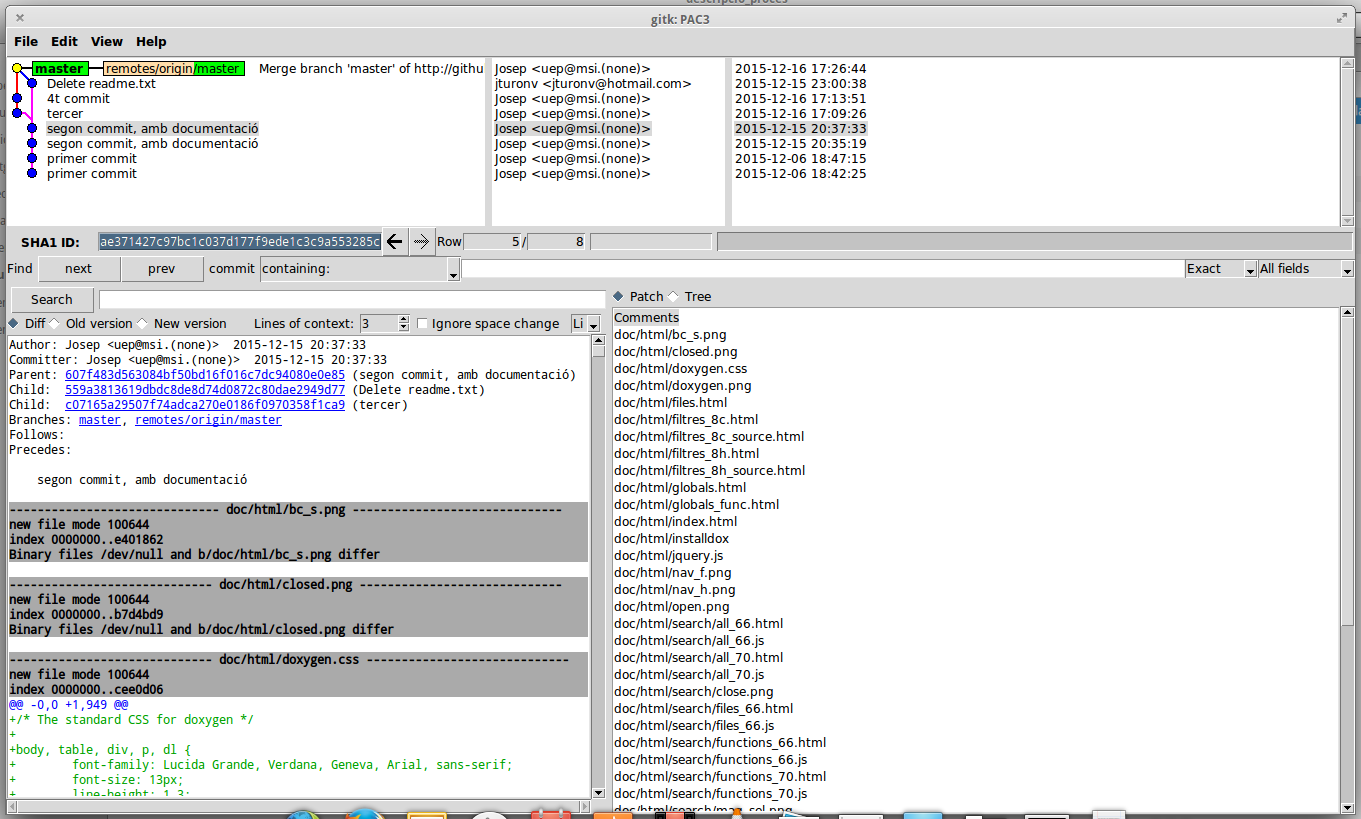
\includegraphics[width=300pt]{gitk}
\caption{Ús de gitk}
\label{fig:gitk}
\end{figure}
\newpage

\section{Documentació}
En un primer apartat, generarem la documentació del codi font filtres i la seva capçalera mitjançant l'eina \textbf{Doxygen}. Comencem instal·lant-la: \bigskip

\qquad sudo apt-get install doxygen\bigskip

Després hem de crear el fitxer de configuració, que contindrà multitud d'opcions per a la creació de la documentació:\bigskip

\qquad doxygen -g configdoxy\bigskip

Modifiquem el nom del projecte, versió, etc., configurem que l'exportació volem fer-la en HTML i LaTeX, l'optimitzem per llenguatge C (ja que és l'únic que utilitzem en el codi), configurem els directoris d'entrada (on es troba el codi) libsrc i sortida (on es desaran els fitxers de documentació) doc, etc. També podem instal·lar la utilitat \textbf{Doxywizard} per a crear o modificar aquest fitxer de configuració amb una interfície gràfica. Amb aquesta eina hem acabat de modificar algun altre paràmetre del fitxer, per exemple habilitant les referència creuades de codi per a totes les entitats (és a dir, que a l'índex de fitxers, clicant sobre del nom del fitxer et condueixi directament al codi), ja que per defecte ho feia per als fitxers de capçalera .h però no pels .c.\bigskip

I un cop configurat aquest fitxer hem entrat dins els fitxers font dels filtres i afegit els comentaris utilitzant etiquetes doxygen explicant la funció de cada filtre, paràmetres i funcionament del codi, utilitzant descripcions abreujades que indicaran a sota de cada filtre el que realitzen, i una descripció detallada amb l'explicació completa del filtre. La documentació de cada filtre quedarà enllaçat amb el codi font, podent accedir ràpidament a un o altre.\bigskip

Fet això, només queda generar la documentació en HTML com havíem configurat i afegir-la al dipòsit. Per generar-la només cal executar la comanda:\bigskip

\qquad doxygen configdoxy\bigskip

I es crearà el directori doc amb dos directoris, un anomenat html amb la documentació en aquest format i un altre, latex, per poder-la crear utilitzant aquesta eina. Si accedim al directori html, només cal obrir el fitxer index.html amb un navegador web per a consultar la documentació generada.\bigskip

Acabem afegint al dipòsit aquest directori doc amb la documentació, i actualitzant els fitxers de codi ja existents amb les últimes versions:\bigskip

\qquad git add libsrc\bigskip

\qquad git add doc\bigskip

Afegim els dos directoris i tots els fitxers que contenen. Amb git status veiem els fitxers nous que s'afegiran al fer el \textit{commit}:\bigskip

\qquad git commit -m "segon commit, amb documentació"\bigskip

I ja només queda actualitzar també el dipòsit remot a GitHub, fent un \textit{push} del local:\bigskip

\qquad git push origin master\bigskip

La segona part consisteix en documentar en un fitxer mitjançant el processador de textos \textbf{LaTeX} el treball desenvolupat en aquesta pràctica (aquest fitxer). Això ho farem amb text pla sense format, utilitzant etiquetes pròpies de LaTeX que el programa compilarà per a obtenir el text en el format escollit (en el nostre cas hem escollit fer-ho com un article).\bigskip

Comencem a instal·lar LaTeX amb el nombre màxim d'opcions: \bigskip

\qquad sudo apt-get install texlive-full \bigskip  

Després procedim a editar un fitxer en blanc anomenat PAC3.tex ubicat dins el directori descripcio\_proces. Configurem algunes opcions com la llengua (català), tipus de codificació de caràcters, tipus de document (article) i l'opció per poder utilitzar els accents i caràcters especials catalans normalment. Definim el títol, autor i data, els diferents apartats que el composen, i comencem a redactar el document. \bigskip
    
Un cop finalitzat el compilem fent:\bigskip

\qquad latex PAC3.tex\bigskip

generant així un fitxer dvi, que podem visualitzar en format gràfic amb l'eina xdvi:\bigskip

\qquad xdvi PAC3.dvi\bigskip

Com que també volem tenir el fitxer en format pdf, el creem executant:\bigskip

\qquad pdflatex PAC3.tex\bigskip

I per acabar, només resta pujar el directori descripcio\_proces amb aquesta documentació als dipòsits local i remot. Fem:\bigskip

\qquad git add descripcio\_proces \bigskip

\qquad git commit -m "final de projecte"\bigskip

\qquad git push origin master \bigskip

Tot i que no l'hem utilitzat per a crear el fitxer, hem provat també l'eina \textbf{LyX}, un editor de textos WYSIWYG (What-You-See-Is-What-You-Get) que permet visualitzar el codi editat amb format mentre es va desenvolupant sense necessitat de compilació final (com sempre, cal instal·lar-lo abans fent sudo apt-get install lyx).
\newpage
\section{Conclusions}
En la realització d'aquesta pràctica hem assolit els següents objectius: \bigskip

A la primera part hem aprés a utilitzar un sistema de control de versions i a diferentciar-ne els dipòsits locals i remots. En el nostre cas hem utilitzat Git, el qual treballa amb una còpia local, en la qual els fitxers afegits van a parar a l'\textit{staging area} que són pujats al dipòsit (local) fent un \textit{commit}. Podem també crear un dipòsit remot, per exemple a GitHub, disponible perquè altres usuaris el puguin clonar com a còpia local. \bigskip

A la segona part, hem aprés a utilitzar Doxygen, un sistema de creació de documentació integrada amb el codi font i exportable a diversos formats, entre ells HTML, per tal de generar automàticament una documentació de tot el codi desenvolupat amb referències creuades entre tots els fitxers del projecte. \bigskip

Finalment, a la tercera part hem aprés a redactar documents amb el processador de textos LaTeX i a diferenciar-ne el contingut del disseny final, ocupant-nos només de redactar aquest contingut i deixant que l'eina compili els codis introduïts amb el text per a crear-ne automàticament el disseny del document, segons el tipus escollit i indicat. \bigskip

\end{document}